\documentclass[solution, letterpaper]{cs121}

\usepackage{graphicx}

\newcommand{\solncolor}{red}
\begin{document}

\header{3}{April 30, 2013, at 11:40 AM}{}{}

%%%%%%%%%%%%%%%%%%%%%%%%%%%%%%%%%%%%%%%%%%%%%%%%%%%%
\section*{Dynamic Programming Approach}
TODO


\section*{Karmarkar-Karp Runtime}
\hspace{4mm} Assuming the values in $A$ are small enough that arithmetic operations take one step, the Karmarkar-Karp algorithm can be implemented in $O(n \log{n})$ steps by using a max-heap. We take an array containing the sequence $A$ and turn it into a max-heap using the standard algorithm, which takes time $O(n \log{n})$. At each step of the iteration, we remove the two largest elements in the heap, which takes time $O(2 \log{n})$. Finding the absolute difference between the elements and adding them back into the heap takes time $O(\log{n})$. At most we conduct these last two steps $n/2$ times, which is on the order of $O(n \log{n})$. Therefore, the algorithm takes $O(n \log{n})$ time overall.

\section*{Experimental Results}
\hspace{4mm} The \texttt{kk.py} file implements the Karmarkar-Karp algorithm and prints out the result for any arbitrary input file. We chose to implement the three local search algorithms in a separate file, \texttt{localsearch.py}. This file generates 50 random instances of the number partition problem, and runs each algorithm and representation combination on each problem. On each iteration, the file outputs the results for each column in the table below; these outputs were formatted for \LaTeX, for our convenience. \texttt{localsearch.py} also writes to an output file, \texttt{graph\_output.txt}, with the remaining residue for each algorithm after every 100 iterations. This data was used to generate the graphs of residue over iterations, on the page after the table.

The following table lists the residuals given by each requested approach, for 50 random instances. On both the table and the following graphs, $KK$ denotes Karmarkar-Karp, $RR$ denotes Repeated Random, $HC$ denotes Hill Climbing, $SA$ denotes Simulated Annealing, and the prefix $PP$ denotes the fact that the prepartitioning representation was used.

\begin{center}
\begin{tabular}{ c |c c c c c c c}
   & $KK$ & $RR$ & $HC$ & $SA$ & $PPRR$ & $PPHC$ & $PPSA$  \\
   \hline
1 & 91427 & 406443511 & 33120495 & 106819349 & 7 & 25 & 183 \\
2 & 63283 & 1322701821 & 362972551 & 35642873 & 133 & 1368 & 16 \\
3 & 163041 & 93821615 & 742852931 & 157347421 & 505 & 904 & 10 \\
4 & 466207 & 12169019 & 425819983 & 80189599 & 173 & 203 & 91 \\
5 & 79396 & 92608552 & 1288477952 & 165452038 & 14 & 669 & 413 \\
6 & 354912 & 50143172 & 28740116 & 13372450 & 334 & 476 & 38 \\
7 & 504732 & 117424542 & 1939594240 & 2658604 & 12 & 852 & 146 \\
8 & 2427505 & 38227327 & 19063717 & 116059393 & 45 & 3752 & 28 \\
9 & 295062 & 124982314 & 15396276 & 39236998 & 144 & 1297 & 3 \\
10 & 54487 & 105614619 & 80998711 & 3028187 & 159 & 28 & 120 \\
11 & 472160 & 610554254 & 148668126 & 502410648 & 16 & 274 & 366 \\
12 & 193792 & 223582218 & 145309958 & 634207712 & 40 & 320 & 170 \\
13 & 88942 & 2629020 & 281037788 & 106171114 & 38 & 210 & 88 \\
14 & 744435 & 174778463 & 556639737 & 98844361 & 309 & 966 & 780 \\
15 & 103848 & 213825332 & 423850736 & 77765850 & 196 & 6552 & 62 \\
16 & 236759 & 187639653 & 612563149 & 47176221 & 231 & 127 & 109 \\
17 & 40674 & 163072572 & 269202562 & 678378576 & 146 & 173 & 47 \\
18 & 11607 & 97594747 & 63574105 & 1115642287 & 29 & 423 & 31 \\
19 & 206345 & 336398345 & 241835911 & 261384795 & 377 & 228 & 404 \\
20 & 144220 & 171380008 & 147280714 & 211426364 & 74 & 316 & 466 \\
21 & 179183 & 56841275 & 215627505 & 34772327 & 711 & 1175 & 833 \\
22 & 547724 & 109350376 & 746490910 & 895155752 & 34 & 1594 & 676 \\
23 & 18603 & 47037011 & 249169143 & 22661999 & 57 & 536 & 54 \\
24 & 55538 & 98347184 & 952841924 & 180238514 & 364 & 3596 & 456 \\
25 & 250158 & 628183176 & 37787026 & 8068206 & 274 & 1354 & 68 \\
26 & 49573 & 74364503 & 109226183 & 216974149 & 249 & 87 & 113 \\
27 & 22252 & 431902502 & 152102174 & 124785836 & 126 & 166 & 72 \\
28 & 317662 & 192482156 & 158367406 & 97609500 & 40 & 4472 & 8 \\
29 & 398754 & 46841870 & 638127884 & 377046968 & 196 & 371 & 325 \\
30 & 256496 & 40624802 & 734552746 & 52301636 & 58 & 238 & 412 \\
31 & 292734 & 135278880 & 623007776 & 923965820 & 20 & 1361 & 375 \\
32 & 35834 & 277278876 & 121073534 & 408387908 & 140 & 66 & 124 \\
33 & 214098 & 66802796 & 72067434 & 316818602 & 80 & 238 & 324 \\
34 & 86784 & 89496906 & 609371060 & 887727188 & 86 & 313 & 89 \\
35 & 12991 & 133914399 & 96724547 & 159623497 & 747 & 191 & 69 \\
36 & 475647 & 763046555 & 263310249 & 63586997 & 131 & 237 & 121 \\
37 & 166296 & 316026416 & 214499626 & 6419464 & 184 & 311 & 135 \\
38 & 86289 & 171707805 & 439576957 & 156811839 & 25 & 510 & 28 \\
39 & 301285 & 160285245 & 204811639 & 250547555 & 25 & 88 & 282 \\
40 & 1181594 & 203836722 & 234938892 & 15023280 & 200 & 5 & 11 \\
41 & 250436 & 212086428 & 900111716 & 104629314 & 86 & 613 & 29 \\
42 & 827960 & 180641356 & 51438100 & 772114620 & 266 & 98 & 332 \\
43 & 775095 & 353128717 & 199636161 & 723722829 & 199 & 894 & 146 \\
45 & 299169 & 380575959 & 1006943279 & 662677875 & 1 & 6293 & 69 \\
44 & 216304 & 434131204 & 593919092 & 40518992 & 0 & 270 & 206 \\
46 & 34292 & 493256096 & 203807418 & 39013290 & 118 & 14 & 320 \\
47 & 121705 & 5488317 & 137323677 & 193375229 & 177 & 202 & 28 \\
48 & 572099 & 104463749 & 624225553 & 212992145 & 221 & 429 & 861 \\
49 & 130764 & 393339398 & 699410876 & 23561622 & 100 & 1 & 57 \\
50 & 83224 & 476586246 & 33612740 & 230095668 & 46 & 208 & 6 \\ \hline
Mean & 300067.54 & 232458760.58 & 383022059.7 & 253088869.22 & 158.86 & 901.88 & 204.0 \\
\end{tabular}
\end{center}

\begin{center}
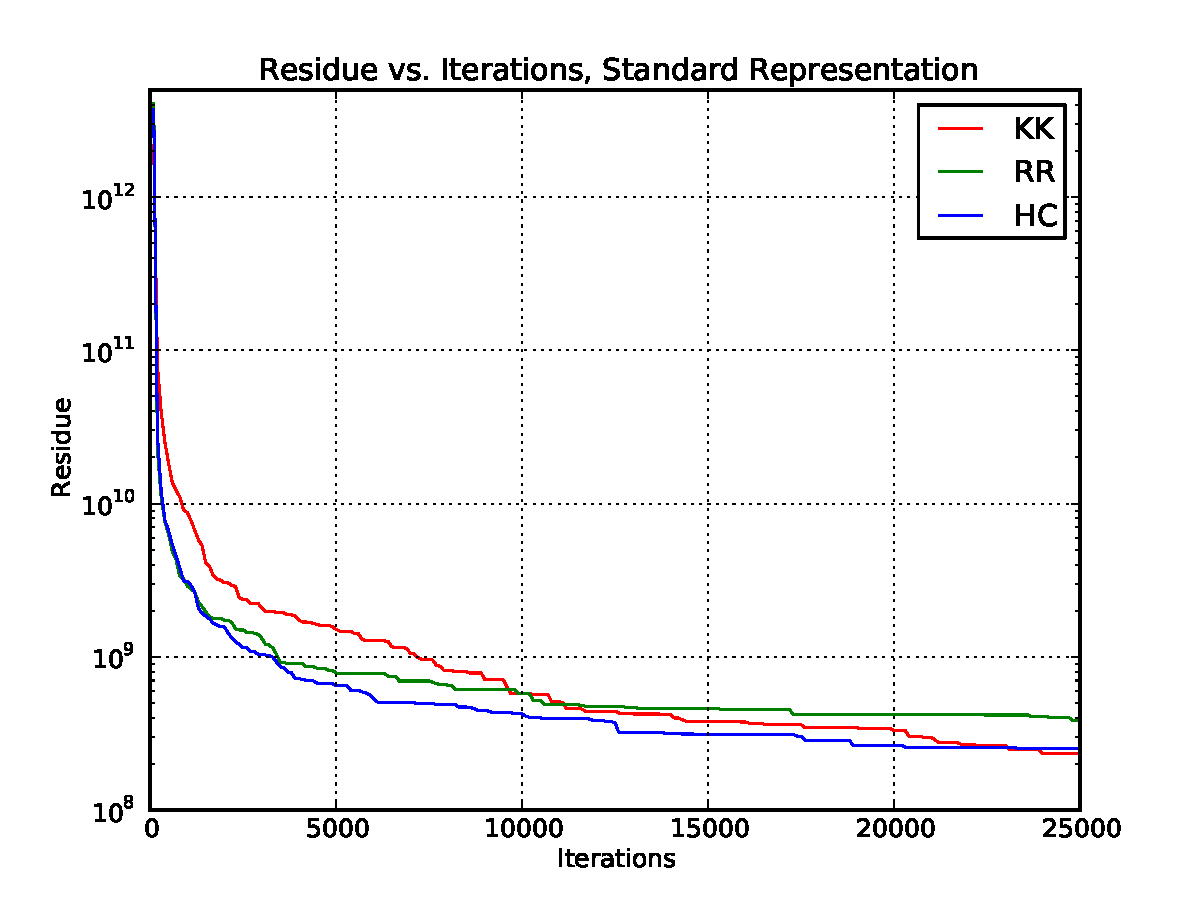
\includegraphics[scale=0.72]{residue-v-iteration-standard.pdf}
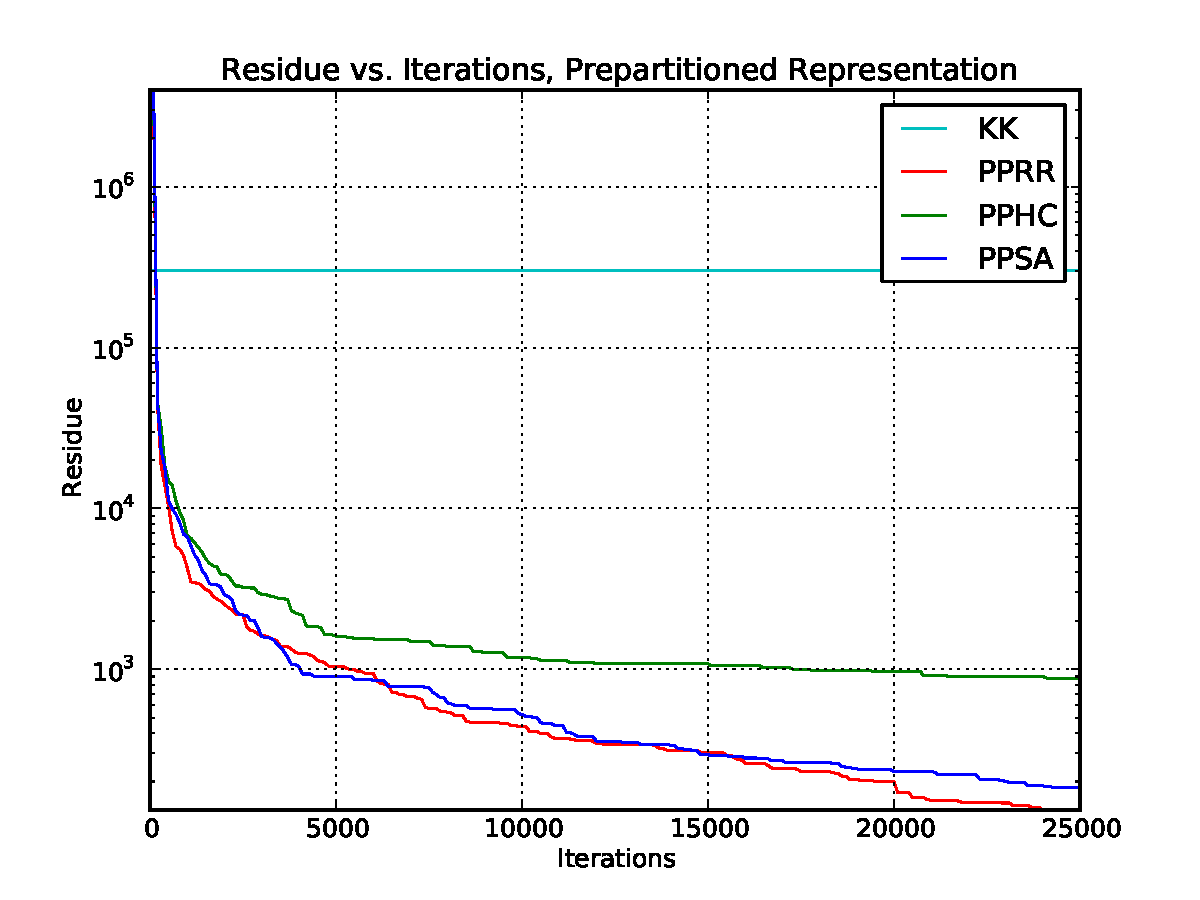
\includegraphics[scale=0.72]{residue-v-iteration-prepartition.pdf}
\end{center}

\section*{Discussion}
\hspace{4mm} We begin by comparing the results of the two representations of the Number Partition problem, then comparing results for each local search algorithm within both representations.

The result residues for the standard representation are significantly worse than those for prepartitioning. They are also significantly worse that the residues returned by the Karmarkar-Karp algorithm. The performance of all the local search algorithms likely suffers because the standard representation insists on partitioning the sequence $A$ into two parts from the very beginning, whereas the prepartitioning result allows elements to be grouped into up to $n$ sets, where $n$ is the number of elements in $A$. This allows for more generality in representing partitions of the set, and results in far more progress when we use the local search algorithms.

For both representations, the repeated random and simulated annealing algorithms returned solutions with approximately equal residues. The repeated random algorithm slightly outperformed the simulated annealing algorithm, likely because we used so many iterations (25,000) that the algorithm was able to eventually generate a very good solution. In the prepartitioning representation, this approach succeeded because of the nature of the representation: on each iteration, the $x_i$ were grouped into up to $n$ different sets, allowing for very different sets to be generated on each iteration. 

The hill climbing algorithm underperformed the other two local search algorithms, likely due to the main flaw with hill climbing algorithms: the possibility of getting stuck at local minima. Although the hill climbing approach was very successful on some iterations, on others it stalled and was unable to escape from a local minimum it found. This phenomenon is clear on the prepartitioning graph. On average across 50 trials, the hill climbing algorithm tended to level off after about 5000 iterations. 

As expected, the simulated annealing algorithm was able to avoid the problem of the hill climbing algorithms. The SA algorithm implements the same general approach as hill climbing, but sometimes randomly moves to a worse location, with probability degrading over time. This avoids the pitfall of hill climbing. Even if the simulated annealing algorithm gets stuck at a local minimum for some time, it will escape from that minimum with some probability. This leads to far better results than hill climbing alone.

We could use a solution from the Karmarkar-Karp as a starting point for either the hill climbing or simulated annealing algorithms. The randomized algorithm simply generates a new solution every time, so having a different starting point would not make a difference in its results, unless the randomly generated results were always worse than the KK result (as is the case with the standard representation). Hill climbing and simulated annealing, on the other hand, rely on iteratively decreasing the residue; as a result, picking a better starting point will give the algorithms a leg up in the process of iterating to a better solution. In particular, the standard representation algorithms could have achieved much better results if they began with the KK result. The results for the prepartitioning representation would likely have been similar in the end, but could have been achieved in significantly fewer iterations.

\end{document}